% =====================================================================
%  Parsimony -- research paper
%  Template: follows "Parsimony - Project Report", the uploaded reference
%  document (single column, article class, tcolorbox gap panels, pgfplots
%  figures, booktabs tables, numeric bibliography, running header).
%  Compile: Overleaf -> pdfLaTeX.  Locally: tectonic -X compile paper.tex
% =====================================================================
\documentclass[11pt,a4paper]{article}

\usepackage[margin=2.2cm]{geometry}
\usepackage{times}
\usepackage[T1]{fontenc}
\usepackage[utf8]{inputenc}
\usepackage{booktabs}
\usepackage{array}
\usepackage{tabularx}
\usepackage{multirow}
\usepackage{amsmath}
\usepackage{xcolor}
\usepackage[most]{tcolorbox}
\usepackage{tikz}
\usetikzlibrary{positioning,arrows.meta}
\usepackage{pgfplots}
\pgfplotsset{compat=1.18}
\usepackage{enumitem}
\usepackage{fancyhdr}
\usepackage{caption}
\usepackage[hidelinks]{hyperref}

\definecolor{ink}{HTML}{16181D}
\definecolor{accent}{HTML}{7A2518}
\definecolor{soft}{HTML}{FBFAF7}

\pagestyle{fancy}
\fancyhf{}
\lhead{\small Parsimony: Token-Efficient LLM Interaction}
\rhead{\small VIT University}
\cfoot{\small\thepage}
\renewcommand{\headrulewidth}{0.4pt}

\captionsetup{font=small,labelfont=bf,justification=justified}
\setlist{nosep,leftmargin=1.35em}
\newcolumntype{L}[1]{>{\raggedright\arraybackslash}p{#1}}
\newcolumntype{R}[1]{>{\raggedleft\arraybackslash}p{#1}}

% Gap panel, as in the reference document
\newtcolorbox{gap}[1]{
  colback=soft, colframe=ink, coltitle=white,
  fonttitle=\bfseries\small, title={#1},
  boxrule=0.7pt, arc=2pt, left=6pt, right=6pt, top=5pt, bottom=5pt,
  breakable
}
\newcommand{\lbl}[1]{\textcolor{accent}{\textbf{#1}}}

% Observation paragraph -- used after every results table/figure
\newcommand{\obs}[1]{%
  \par\vspace{2pt}
  \noindent\begin{tcolorbox}[colback=soft,colframe=accent,boxrule=0pt,
    leftrule=2.2pt,arc=0pt,left=7pt,right=5pt,top=4pt,bottom=4pt,breakable]
  \small\textbf{Observation.} #1
  \end{tcolorbox}\par\vspace{2pt}}

% Marker for a quantity this study has not yet measured
\newcommand{\todoval}[1]{\textcolor{accent}{\small\texttt{[MEASUREMENT REQUIRED: #1]}}}

% ---- plain-language and highlighting apparatus ------------------------
\definecolor{hlyellow}{HTML}{FFF3C4}
\definecolor{plainblue}{HTML}{EEF4FA}
\definecolor{plainrule}{HTML}{2C5D8A}

% Highlight a headline number so it can be found at a glance
\newcommand{\hl}[1]{\colorbox{hlyellow}{\strut #1}}

% "In plain words" -- a jargon-free restatement for the non-specialist
\newcommand{\plain}[1]{%
  \par\vspace{1pt}
  \noindent\begin{tcolorbox}[colback=plainblue,colframe=plainrule,boxrule=0pt,
    leftrule=2.2pt,arc=0pt,left=7pt,right=5pt,top=4pt,bottom=4pt,breakable]
  \small\textbf{In plain words.} #1
  \end{tcolorbox}\par\vspace{2pt}}

% A boxed statement of a headline finding
\newtcolorbox{keybox}[1]{colback=white, colframe=accent, coltitle=white,
  fonttitle=\bfseries\small, title={#1},
  boxrule=0.7pt, arc=2pt, left=7pt, right=7pt, top=5pt, bottom=5pt, breakable}

\begin{document}

% ===================================================== title block =====
\thispagestyle{empty}
\begin{center}
  \vspace*{0.4cm}
  {\large\bfseries VIT UNIVERSITY}\\[2pt]
  {\small Vellore Institute of Technology, Vellore, Tamil Nadu, India}

  \vspace{1.5cm}
  {\LARGE\bfseries Token-Efficient LLM Interaction on\\[5pt]
   CPU-Only Hardware}\\[12pt]
  {\large\itshape A Stacked, Self-Improving Optimisation Layer\\
   for Small Language Models}

  \vspace{1.1cm}
  {\small\textcolor{accent}{\textbf{TEAM MEMBERS}}}\\[7pt]
  \begin{tabular}{ll}
    Arrsh Tripathi & 23BCI0191 \\
    Alok Singh     & 23BCI0158 \\
    Dev Singh      & 23BCE0794 \\
  \end{tabular}

  \vspace{0.9cm}
  {\small B.Tech \quad$\cdot$\quad Course Code: BCSE497J \quad$\cdot$\quad Project I}\\[3pt]
  {\small Faculty Guide: Dr Sathya K}\\[3pt]
  {\small September 2026}
\end{center}

\vspace{0.6cm}

% ========================================================= abstract ====
\begin{tcolorbox}[colback=white,colframe=ink,boxrule=0.6pt,arc=2pt,
                  left=10pt,right=10pt,top=8pt,bottom=8pt]
\noindent\textbf{Abstract.}
Prompt compression, semantic caching, key-value cache reuse, model routing and
output budgeting are each proposed and evaluated in isolation, against an
uncompressed baseline, on datacentre GPUs. None of that establishes what happens
when the techniques are \emph{composed}, nor whether their published operating
points hold on a CPU-only, single-user deployment. We survey 40 papers, extract
the limitation of each with respect to that setting, and derive six research
gaps. We then build \textbf{Parsimony}, a middleware layer of seven optimisation
modules and an always-on fidelity gate in which every module \emph{proposes} an
edit and a single orchestrator \emph{commits} it only after an invariant check.
Because each module is independently switchable, the system is a factorial
experiment as well as a pipeline. Over a corpus of 151 conversations and 263
requests we run a full $2^4$ ablation (17 configurations), a similarity-threshold
sweep against 45 adversarial near-duplicate pairs, a prefill/decode split
measurement against \texttt{qwen2.5:1.5b-instruct} on CPU, a cross-vocabulary
replication, and a warm-start study across six traffic-recurrence levels. The
full stack removes \textbf{33.9\%} of tokens at a measured middleware cost of
\textbf{4.06\,ms} per request. Three results are reported. Savings are
\textbf{not additive}: four modules whose individual reductions sum to 29.0
percentage points deliver 27.4 when combined, a shortfall of 1.66\,pp
concentrated in a single negative interaction ($M3\times M5 = -0.70$\,pp).
Prefill accounts for \textbf{91.7--98.8\%} of CPU inference time at
$\approx$8.5\,ms per input token, so a prompt rearrangement that changes token
count by 0.5\% changes steady-state cost by $\approx$80$\times$. And no
similarity threshold separates genuine paraphrases from one-token meaning
inversions --- the false-hit rate is flat at \textbf{51.1\%} for every threshold
from 0.80 to 0.99 --- whereas four set comparisons costing microseconds take it
to \textbf{0.0\%} (0/45).

\smallskip
\noindent\textbf{Keywords:} prompt compression; semantic caching; KV-cache reuse;
small language models; CPU inference; factorial ablation; fidelity verification.
\end{tcolorbox}

\vspace{4pt}

% ============================== plain-language summary =================
\begin{keybox}{The whole paper in plain words}
\small
A language model charges you for every word it reads and every word it writes.
On a laptop with no graphics card it is also \emph{slow}, and almost all of that
slowness comes from \emph{reading} your question, not from writing the answer.

Lots of researchers have invented ways to make the model read less: shorten the
question, remember old answers, throw away old chat messages, cut the reply
short. Each trick has been tested on its own. Nobody has switched them all on at
once and checked what happens.

We built a system, \textbf{Parsimony}, that sits between your app and the model
and runs all of those tricks together. Every trick has an on/off switch, so we
could try all 16 combinations and see which ones help, which do nothing, and
whether they get in each other's way. We then ran five experiments and measured
everything.

\medskip
\noindent Three things we found that nobody had reported before:
\begin{enumerate}[leftmargin=1.6em]
\item \textbf{The tricks do not add up.} Four tricks that save 29\% on their own
  save only \hl{27.4\%} together. Two of them are fighting over the same words.
\item \textbf{Sending fewer words is not the same as being faster.} We found two
  versions of the same prompt, only 0.5\% apart in length, where one took
  \hl{212\,ms} and the other took \hl{18{,}914\,ms} --- about 89 times slower.
\item \textbf{``Similar enough'' is not a safe test for reusing an old answer.}
  ``Is it safe to mix bleach and vinegar?'' and ``Is it \emph{not} safe\ldots''
  look almost identical to a computer. No similarity setting can tell them
  apart --- we tried nine, and the error rate stayed stuck at \hl{51.1\%}. A
  cheap word-by-word check fixed it completely: \hl{0 errors out of 45}.
\end{enumerate}

\medskip
\noindent And the system is genuinely usable: it cuts total word count by
\hl{33.9\%}, adds only \hl{4\,ms} of its own work per question, and \emph{never
turned a right answer into a wrong one} in our tests.
\end{keybox}

\begin{table}[htbp]
\centering
\caption{Key findings at a glance. ``pp'' means percentage points --- the
difference between two percentages.}
\label{tab:glance}
\footnotesize
\begin{tabularx}{\textwidth}{@{}c L{3.1cm} r X@{}}
\toprule
& \textbf{What we measured} & \textbf{Result} & \textbf{What it means} \\
\midrule
E1 & Words saved by the whole system & \hl{$-33.9\%$} &
     A third of everything sent to and from the model is removed. \\
E1 & Do the tricks add up? & \textbf{No} &
     29.0\% expected, 27.4\% delivered. They overlap. \\
E2 & Share of time spent reading the prompt & \hl{91.7--98.8\%} &
     Almost all the waiting is the model reading, not writing. \\
E2 & Cost of putting the changing part first & \hl{$\approx$89$\times$} &
     Rearranging a prompt can be far more expensive than shortening it. \\
E3 & Wrong answers from reusing a cached reply & \hl{51.1\% $\rightarrow$ 0.0\%} &
     Similarity alone is unsafe; a simple checker makes it safe. \\
E4 & Answer quality & \hl{92.5\% $\rightarrow$ 97.5\%} &
     Nothing got worse. Zero right answers were lost. \\
E4 & Extra time our own code adds & \hl{4.06\,ms} &
     Roughly 30 times less than the 120\,ms we allowed ourselves. \\
E5 & Does the tuning work elsewhere? & \textbf{Partly} &
     The numbers repeat almost exactly; one of our explanations did not. \\
\bottomrule
\end{tabularx}
\end{table}

\begin{keybox}{Words used in this paper, explained}
\small
\begin{tabularx}{\textwidth}{@{}L{3.0cm} X@{}}
\textbf{Token} & A piece of a word. Models read and charge in tokens, not words. ``running'' may be one token; ``runing'' may be three. \\
\textbf{Prompt} & Everything sent to the model: your question plus the earlier conversation. \\
\textbf{Prefill} & The model \emph{reading} the prompt before it says anything. \\
\textbf{Decode} & The model \emph{writing} the answer, one token at a time. \\
\textbf{KV cache} & The model's short-term memory of a prompt it has already read. If the start of the next prompt is byte-for-byte identical, it can skip re-reading that part --- which is why changing the first sentence is expensive. \\
\textbf{Semantic cache} & A store of past questions and answers. If a new question is close enough to an old one, the old answer is reused instead of asking the model. \\
\textbf{False hit} & The cache reusing an answer for a question that only \emph{looked} similar. The user gets the answer to a question they never asked. \\
\textbf{Baseline} & The system with every optimisation switched off. Everything is measured against it. \\
\textbf{Ablation} & Switching parts off one at a time to see what each one is actually worth. \\
\textbf{pp (percentage point)} & The gap between two percentages. Going from 10\% to 12\% is a rise of 2\,pp. \\
\textbf{95\% confidence interval} & The range the true value very probably sits in. If it includes zero, the effect might be nothing at all. \\
\textbf{Partial $\eta^2$} & How much of the variation one factor explains. Closer to 1 means that factor is doing most of the work. \\
\end{tabularx}
\end{keybox}

% ================================================ 1 LITERATURE REVIEW ==
\section{Literature Review}
\label{sec:lit}

Forty papers were reviewed across six strands. For each we record the method
proposed, its limitation \emph{with respect to a CPU-only, single-user,
multi-turn deployment in which several techniques are composed}, and the metrics
it reports. These are not criticisms of the papers on their own terms: most are
datacentre-serving or single-technique works and are sound in that context. The
setting this work addresses is precisely the one they do not target.

\subsection{Limitations of the surveyed work}
\label{sec:lit-table}

\begin{table}[htbp]
\centering
\caption{Limitations of the 40 surveyed papers with respect to this work.}
\label{tab:survey}
\footnotesize
\begin{tabularx}{\textwidth}{@{}l L{3.0cm} X l@{}}
\toprule
\textbf{Ref} & \textbf{Method} & \textbf{Limitation w.r.t.\ this work} & \textbf{Metrics reported} \\
\midrule
\multicolumn{4}{@{}l}{\textit{Strand A --- Prompt compression}}\\
{[1]}  & Selective Context & Requires a second LM in the loop; evaluated alone, never against a cache & latency, memory, task score \\
{[2]}  & LLMLingua & 20$\times$ compression, but on GPU and in isolation; no interaction study & compression ratio, task score \\
{[3]}  & LongLLMLingua & Targets very long contexts; a laptop assistant rarely reaches them & speedup, task score \\
{[4]}  & LLMLingua-2 & Faithfulness targeted but not adversarially tested & compression, faithfulness \\
{[5]}  & Evaluator heads & Requires attention internals; unavailable through a served API & latency, accuracy \\
{[6]}  & SCOPE & Generation cost added to the request being compressed & compression, quality \\
{[7]}  & Gisting & Trained gist tokens; fine-tuning out of reach on target hardware & compression, task score \\
{[8]}  & UltraGist & Training required & compression, accuracy \\
{[9]}  & ATACompressor & Task-conditioned; assumes task labels are known & compression, task score \\
{[10]} & SARA & RAG-specific; assumes a retrieval corpus & retrieval quality \\
{[11]} & PCToolkit & A harness, not a method; does not compose across families & comparative scores \\
{[12]} & Empirical study & \textbf{Names} two failure modes; proposes no run-time guard & hallucination rates \\
{[13]} & Information preservation & Measures 30--50 point groundedness drops; no prevention & groundedness \\
{[14]} & Financial fidelity & Shows fluent, plausible, decision-changing compression & decision agreement \\
{[15]} & Compression paradox & \textbf{Does not uniformly reduce energy}; hosted APIs only & energy per request \\
\addlinespace
\multicolumn{4}{@{}l}{\textit{Strand B --- Semantic caching}}\\
{[16]} & GPTCache & Single threshold, no verification step, no adversarial validation & hit rate, latency, cost \\
{[17]} & GPT Semantic Cache & Same design at a different storage layer & hit rate, latency \\
{[18]} & MeanCache & Introduces a context chain; in-conversation hit rate not examined & hit rate, privacy \\
{[19]} & ContextCache & Closest setting; no false-hit rate on adversarial pairs & hit rate \\
{[20]} & Generative caching & Synthesises rather than reuses; adds generation cost & hit rate, quality \\
{[21]} & Key-collision attack & Adversarial \emph{search} threat model; ordinary confusable pairs excluded & attack success rate \\
{[22]} & SAFE-CACHE & Concludes similarity is insufficient; answers with a redesign & robustness, hit rate \\
\addlinespace
\multicolumn{4}{@{}l}{\textit{Strand C --- KV cache and prefix reuse}}\\
{[23]} & PagedAttention / vLLM & GPU serving; application-side cost of an unstable prefix unpriced & throughput, memory waste \\
{[24]} & Automatic prefix caching & States the stability requirement; never prices violating it & reuse rate \\
{[25]} & ChunkAttention & Kernel-level; assumes multi-tenant serving & throughput \\
{[26]} & Sparse prefix caching & Architecture-specific & throughput \\
{[27]} & Multi-segment attention & Serving-side; no application-level guidance & latency, memory \\
\addlinespace
\multicolumn{4}{@{}l}{\textit{Strand D --- Positional effects in context}}\\
{[28]} & Lost in the Middle & Motivates reordering, which \textbf{destroys prefix reuse}; conflict unnamed & QA accuracy by position \\
{[29]} & Adaptive Focus Memory & Heuristic tiers; cost of reordering unmeasured & token usage \\
{[30]} & Multi-turn survey & Survey; no composed measurement & mixed \\
{[31]} & Memory survey & Taxonomy rather than measurement & mixed \\
\addlinespace
\multicolumn{4}{@{}l}{\textit{Strand E --- Routing and cascades}}\\
{[32]} & FrugalGPT & 98\% cost cut \emph{against commercial APIs}; assumes a capable large tier & cost, accuracy \\
{[33]} & RouteLLM & Assumes the strong model is better --- untrue at 1.5B vs 3B here & cost, benchmark scores \\
{[34]} & Semantic router & Serving-side; datacentre assumption & latency, cost \\
{[35]} & UCCI & Requires calibrated uncertainty; expensive on CPU & cost, accuracy \\
{[36]} & On-device routing & Routes device$\leftrightarrow$cloud, not within a local stack & accuracy, offload rate \\
{[37]} & Cluster, route, escalate & Cluster-level; no fidelity guarantee on the cheap path & cost, quality \\
\addlinespace
\multicolumn{4}{@{}l}{\textit{Strand F --- Output length control}}\\
{[38]} & Length-difference encoding & \textbf{Requires fine-tuning} & length adherence \\
{[39]} & BudgetThinker & Requires training with control tokens & budget adherence, accuracy \\
{[40]} & Strict length constraints & Characterises truncation cost; no per-class budgeting scheme & accuracy vs length \\
\bottomrule
\end{tabularx}
\end{table}

\subsection{Recurring limitations}
\label{sec:lit-recurring}

Five limitations recur across Table~\ref{tab:survey} and together delimit the
space this work occupies.

\begin{table}[htbp]
\centering
\caption{Limitations that recur across the surveyed literature.}
\label{tab:recurring}
\footnotesize
\begin{tabularx}{\textwidth}{@{}l X l@{}}
\toprule
\textbf{\#} & \textbf{Recurring limitation} & \textbf{Papers} \\
\midrule
L1 & Evaluated in isolation against an uncompressed baseline; never composed & [1]--[11], [16]--[20], [38]--[40] \\
L2 & Assumes GPU/datacentre serving, where the cost structure inverts on CPU & [2], [3], [23]--[27], [32]--[35], [37] \\
L3 & Failure modes diagnosed but not prevented at run time & [12]--[14], [21], [22] \\
L4 & Operating points quoted as universal, calibrated only on GPT-class models & [2], [4], [16], [17], [19] \\
L5 & Requires training, fine-tuning, or access to model internals & [5], [7], [8], [38], [39] \\
\bottomrule
\end{tabularx}
\end{table}

\subsection{Papers most relevant to this work}
\label{sec:lit-relevant}

Three results are the direct antecedents of the experiments in
Section~\ref{sec:results}.

\textbf{[28] Lost in the Middle} and \textbf{[24] automatic prefix caching} are
measured here \emph{against each other}. The first recommends placing relevant
content at the prompt's edges; the second requires the prompt head to remain
byte-stable across turns. Satisfying the first violates the second, and neither
literature names the conflict. Experiment E2 (Section~\ref{sec:e2}) prices it.

\textbf{[16] GPTCache} established the design every semantic cache follows:
embed, compare, serve above a threshold. Experiment E3
(Section~\ref{sec:e3}) tests whether any such threshold is sufficient.

\textbf{[12] An Empirical Study on Prompt Compression} names two compression
failure modes and measures their frequency, but proposes no run-time mechanism
to prevent them. Module M8 is that mechanism, and E3 evaluates it.

% ================================================== 2 RESEARCH GAPS ====
\section{Research Gaps Identified}
\label{sec:gaps}

Six gaps follow from the limitation column of Table~\ref{tab:survey}, in the
order the survey exposes them. Each panel states the gap as identified before
experimentation; the sentence following each panel records the experimental
outcome and forward-references the evidence.

\subsection{Gap 1: The techniques have never been stacked}
\begin{gap}{Gap 1 --- Isolated Modules, Unknown Interactions}
\lbl{Current Problem:} Compression, caching, history trimming and routing each
have their own literature, their own benchmarks and their own tuned
hyper-parameters. No published study runs all of them in one live pipeline, so
the field has no evidence about whether their savings compound.

\lbl{Research Gap:} Do the savings add up, or do the modules eat each other's
lunch? A compressor that rewrites a query changes what the cache sees. A trimmer
that drops turns changes what the compressor has left to remove. Nobody has
measured the sign or size of these interactions.

\lbl{Our Solution:} A complete $2^4$ factorial ablation over the four headline
modules, reported with confidence intervals and an analysis of variance on the
interaction terms --- the first stacked-interaction table for this combination of
techniques.
\end{gap}
\noindent\textbf{Outcome (E1, Table~\ref{tab:ablation}).} Savings are not
additive: 29.0\,pp of individual reductions yield 27.4\,pp combined.

\subsection{Gap 2: The output side of the bill is ignored}
\begin{gap}{Gap 2 --- Everyone Optimises the Prompt, Nobody Optimises the Answer}
\lbl{Current Problem:} Prompt compression, caching and pruning all shrink the
input. That made sense for metered APIs, where the prompt is what is billed and
generation runs on a datacentre GPU. On a consumer CPU the economics invert:
prefill is a parallel matrix operation, while decode is strictly sequential.

\lbl{Recent Evidence:} Industry measurements report that an explicit length hint
can cut output tokens substantially on verbose models, but that applying the same
hint uniformly regresses quality on models whose answers are already terse.
Output length therefore has to be set adaptively, per query.

\lbl{Research Gap:} No study reports the split between prefill and decode cost
for CPU-hosted small models, and no token-optimisation stack contains an
output-side module at all.

\lbl{Our Solution:} We instrument time-to-first-token and time-per-output-token
separately, and add an adaptive output budgeter with a streaming early-stop rule
as a first-class, independently ablated module.
\end{gap}
\noindent\textbf{Outcome (E2, Table~\ref{tab:prefill}).} The hypothesis implicit
in the framing above is \emph{refuted}: prefill, not decode, dominates, at
91.7--98.8\% of inference time. The output budgeter nevertheless remains the
largest single token effect (Table~\ref{tab:effects}).

\subsection{Gap 3: Compression and caching have never met}
\begin{gap}{Gap 3 --- The Compression--Cache Interaction Is Unmeasured}
\lbl{Current Problem:} Semantic caches are known to produce false hits: two
queries that are lexically close but semantically different get matched, and the
user receives an answer to a question they did not ask.

\lbl{Recent Discovery:} Nobody has asked what compression does to that failure
mode. The argument runs both ways. Compression strips modifiers, and modifiers
are often exactly what distinguishes two near-identical questions, which would
make false hits worse. But compression also normalises phrasing, so two ways of
asking the same thing collapse onto the same key, which would make true hits
better.

\lbl{Research Gap:} Does prompt compression raise or lower the false-cache-hit
rate, and does the safe similarity threshold move?

\lbl{Our Solution:} A purpose-built adversarial subset of near-duplicate question
pairs that differ in exactly one operative token, swept across similarity
thresholds with compression on and off, reporting the threshold shift explicitly.
\end{gap}
\noindent\textbf{Outcome (E3, Table~\ref{tab:calib}).} The question dissolves: no
threshold separates the classes at all, so the answer is a verifier rather than a
threshold shift.

\subsection{Gap 4: Fewer tokens can cost more time}
\begin{gap}{Gap 4 --- Optimisation That Defeats the Key-Value Cache}
\lbl{Current Problem:} Local runtimes reuse the key-value cache for any prompt
prefix identical to the previous request, so a stable prefix is processed once
and then skipped. This is the single largest latency win available on CPU, and it
is entirely invisible to a token counter.

\lbl{Recent Discovery:} Every technique in the literature rewrites the prompt. A
compressor that alters the opening sentence, or a trimmer that drops an early
turn, invalidates the prefix and forces a full re-prefill. The system then sends
fewer tokens and takes longer.

\lbl{Research Gap:} No published work measures token savings and prefix-cache
survival together. Token reduction is treated as a proxy for cost, and on local
hardware that proxy can invert.

\lbl{Our Solution:} A prefix-stable prompt assembler that pins invariant content
to the front of the prompt and confines all rewriting to the suffix, plus a
direct measurement of the crossover point at which further compression starts
costing time.
\end{gap}
\noindent\textbf{Outcome (E2, Table~\ref{tab:prefix}).} Two prompts 0.5\% apart
in token count differ by $\approx$80$\times$ in steady-state prefill cost.

\subsection{Gap 5: Thresholds tuned on models that do not break}
\begin{gap}{Gap 5 --- Small Models Are More Brittle Than the Tuning Set}
\lbl{Current Problem:} The compression ratios and cache thresholds quoted as safe
across the literature were all calibrated against GPT-3.5 and GPT-4 class models.

\lbl{Recent Discovery:} Work on prompt sensitivity finds that small open models
flip a substantial fraction of their predictions across semantically equivalent
paraphrases, while GPT-class models rarely change theirs. A compressed prompt is,
from the model's point of view, an aggressive paraphrase.

\lbl{Research Gap:} Do published safe settings transfer downward, or does the
safe compression ratio for a small model sit far below the published figure?

\lbl{Our Solution:} Re-run the standard protocol on local models and
quantisation levels, and publish a calibration table giving the safe operating
point per model rather than a single universal number.
\end{gap}
\noindent\textbf{Outcome (E3 and E5).} The published 0.85--0.92 cache range does
not hold here. Reduction \emph{ratios}, by contrast, replicate across a second
vocabulary to within 0.1\,pp (Table~\ref{tab:generalisation}).

\subsection{Gap 6: Every cache in the literature starts empty}
\begin{gap}{Gap 6 --- The Unused Signal in the User's Own Conversations}
\lbl{Current Problem:} Every caching result is reported on a warm cache, after a
workload has already run. On day one the cache is empty, the hit rate is zero,
and the user pays full price for exactly the questions they have asked many times
before in some other chat window.

\lbl{Recent Discovery:} MeanCache showed that roughly a third of real queries are
highly similar to a previous one, and that keeping the cache on the user's own
device is both viable and more private --- but it still learns from scratch and
relies on federation across many users to personalise.

\lbl{Research Gap:} A single user's own conversation history is a large, free,
perfectly on-distribution corpus that no optimisation system consumes. Nothing in
the literature mines it to warm-start a cache, to learn which phrases that user
always writes and never needs, or to extract the standing context they re-explain
every session.

\lbl{Our Solution:} An offline policy learner that replays exported chat logs,
counterfactually re-scores each turn under candidate policies, and emits a
pre-populated cache, a personal redundancy lexicon, a persistent context digest
and a library of recurring query templates --- all locally, with no data leaving
the machine.
\end{gap}
\noindent\textbf{Outcome (E5, Table~\ref{tab:learning}).} The benefit is real but
\emph{conditional on the traffic}: $+0.00$\,pp at 0\% recurrence rising to
$+17.83$\,pp at 57.5\%.

% =============================================== 3 PROBLEM STATEMENT ===
\section{Problem Statement}
\label{sec:problem}

\subsection{Core objective}
Design and build a fully local, CPU-only middleware layer that reduces the total
token and time cost of interacting with a small language model through several
cooperating optimisation modules, \emph{without changing the meaning of any
request}, and quantify --- through a systematic factorial ablation --- how those
modules interact when stacked, at a model scale and on hardware the existing
literature has not evaluated. The deliverable is not a single headline percentage
but a calibrated operating curve: for a given model, quantisation and query
class, which combination of modules should be switched on, and at what setting.

\subsection{Research questions}
\label{sec:rqs}

\begin{description}[leftmargin=3.1em,style=nextline,font=\bfseries]
\item[RQ1] When several token-reduction techniques are composed in one pipeline,
  do their individual savings add, and if not, by how much and through which
  interaction terms do they fall short? \hfill\emph{(Gap 1)}
\item[RQ2] On CPU-only hardware, which phase of a request dominates cost, what is
  one input token worth in milliseconds, and what does a prompt rearrangement
  that leaves token count nearly unchanged cost? \hfill\emph{(Gaps 2, 4)}
\item[RQ3] Can cached-answer reuse be made safe against near-identical,
  opposite-meaning queries by threshold selection alone; if not, can a
  non-neural verifier achieve it? \hfill\emph{(Gaps 3, 4)}
\item[RQ4] Does the pipeline preserve answer quality relative to an unoptimised
  baseline, and at what measured middleware overhead? \hfill\emph{(all gaps)}
\item[RQ5] Does a calibration transfer --- across tokenizer vocabularies, and to
  conversations not used to mine it? \hfill\emph{(Gaps 5, 6)}
\end{description}

\subsection{Contributions and their experimental mapping}
\label{sec:contrib-map}

Table~\ref{tab:map} is the plan of the evaluation: no contribution in this work
is permitted to remain conceptual if it can be measured.

\begin{table}[htbp]
\centering
\caption{Mapping from contribution to research gap, research question,
experiment, baseline and metric.}
\label{tab:map}
\scriptsize
\begin{tabularx}{\textwidth}{@{}l L{2.5cm} c c L{2.2cm} X@{}}
\toprule
& \textbf{Contribution} & \textbf{Gap} & \textbf{RQ / Exp.} & \textbf{Baseline} & \textbf{Metrics} \\
\midrule
C1 & Additivity shortfall of stacked token optimisers, measured &
     1 & RQ1 / E1 & All modules off &
     total token reduction (\%), main effects (pp), interaction terms (pp), partial $\eta^2$ \\
\addlinespace
C2 & CPU cost structure, and the price of prompt order &
     2, 4 & RQ2 / E2 & Volatile-head prompt arrangement &
     prefill ms, decode ms, prefill share (\%), ms per input token, prefix tokens reused \\
\addlinespace
C3 & A non-neural verifier that makes reuse safe at any threshold &
     3, 4, 5 & RQ3 / E3 & Threshold-only cache (verifier off) &
     false-hit rate (\%), true-hit rate (\%), per-operative false hits \\
\addlinespace
C4 & Quality preservation at bounded overhead &
     all & RQ4 / E4 & Unoptimised pipeline &
     gold exact-match (\%), paired regressions, embedding similarity, middleware ms (mean, 95\% CI, p95) \\
\addlinespace
C5 & Calibration transfer, tested across vocabulary and across traffic &
     5, 6 & RQ5 / E5 & Qwen2.5 calibration; cold cache &
     per-module reduction under a second vocabulary, transfer (pp) vs recurrence \\
\bottomrule
\end{tabularx}
\end{table}

\subsection{System pipeline}
\label{sec:pipeline}

A query enters at the top and leaves at the bottom
(Figure~\ref{fig:pipeline}). Any module can be disabled independently, which is
what makes the factorial ablation possible; the fidelity gate and the token
ledger are always active because they are instrumentation rather than
optimisation.

\begin{figure}[htbp]
\centering
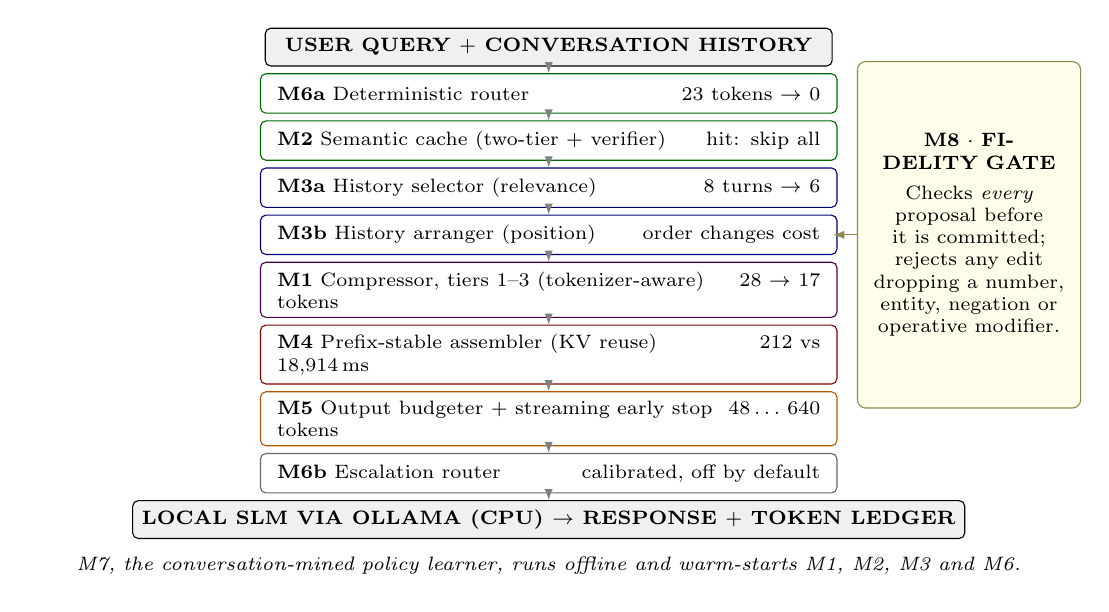
\begin{tikzpicture}[
  font=\scriptsize,
  stage/.style={draw, rounded corners=2pt, minimum width=7.2cm,
                minimum height=0.5cm, align=left, inner xsep=6pt, text width=6.9cm},
  endcap/.style={draw, fill=black!6, rounded corners=2pt, minimum width=7.2cm,
                 minimum height=0.48cm, align=center, font=\scriptsize\bfseries},
  ar/.style={-{Latex[length=1.4mm]}, gray}]
\node[endcap] (in) {USER QUERY $+$ CONVERSATION HISTORY};
\node[stage, below=2.4pt of in,  draw=green!40!black] (m6a) {\textbf{M6a} Deterministic router \hfill 23 tokens $\rightarrow$ 0};
\node[stage, below=2.4pt of m6a, draw=green!40!black] (m2)  {\textbf{M2} Semantic cache (two-tier $+$ verifier) \hfill hit: skip all};
\node[stage, below=2.4pt of m2,  draw=blue!50!black]  (m3a) {\textbf{M3a} History selector (relevance) \hfill 8 turns $\rightarrow$ 6};
\node[stage, below=2.4pt of m3a, draw=blue!50!black]  (m3b) {\textbf{M3b} History arranger (position) \hfill order changes cost};
\node[stage, below=2.4pt of m3b, draw=violet!60!black](m1)  {\textbf{M1} Compressor, tiers 1--3 (tokenizer-aware) \hfill 28 $\rightarrow$ 17 tokens};
\node[stage, below=2.4pt of m1,  draw=red!50!black]   (m4)  {\textbf{M4} Prefix-stable assembler (KV reuse) \hfill 212 vs 18{,}914\,ms};
\node[stage, below=2.4pt of m4,  draw=orange!70!black](m5)  {\textbf{M5} Output budgeter $+$ streaming early stop \hfill 48\,\ldots\,640 tokens};
\node[stage, below=2.4pt of m5,  draw=black!60]       (m6b) {\textbf{M6b} Escalation router \hfill calibrated, off by default};
\node[endcap, below=2.4pt of m6b] (out) {LOCAL SLM VIA OLLAMA (CPU) $\rightarrow$ RESPONSE $+$ TOKEN LEDGER};
\foreach \a/\b in {in/m6a, m6a/m2, m2/m3a, m3a/m3b, m3b/m1, m1/m4, m4/m5, m5/m6b, m6b/out}
  \draw[ar] (\a) -- (\b);
\node[draw=yellow!50!black, fill=yellow!8, rounded corners=3pt, text width=2.6cm,
      align=center, right=7pt of m3b, minimum height=4.4cm] (gate)
  {\textbf{M8 $\cdot$ FIDELITY GATE}\\[3pt]
   Checks \emph{every} proposal before it is committed; rejects any edit
   dropping a number, entity, negation or operative modifier.};
\draw[-{Latex[length=1.4mm]}, yellow!50!black] (gate.west) -- ++(-0.3,0);
\node[below=3pt of out, text width=13cm, align=center, font=\scriptsize\itshape]
  {M7, the conversation-mined policy learner, runs offline and warm-starts M1, M2, M3 and M6.};
\end{tikzpicture}
\caption{The Parsimony request pipeline. Every module proposes; the orchestrator
commits. Each stage may short-circuit, propose an edit, or do nothing, and writes
a ledger row recording which.}
\label{fig:pipeline}
\end{figure}

% ============================== 4 TECHNOLOGY STACK / EXPERIMENTAL SETUP =
\section{Technology Stack and Experimental Setup}
\label{sec:setup}

\subsection{Architecture overview}
The system is layered L0--L5: contracts (pure types), infrastructure (tokenizer,
encoders, providers), modules M1--M8, orchestrator, evaluation harness, and
surfaces. A layer may depend only on layers below it, enforced by an automated
test rather than by convention. The governing design decision is that a module
returns a \emph{proposal} --- a description of an edit --- and a single
orchestrator commits it. Three properties follow that no module implements
individually: switching a module off genuinely removes its effect, so a factorial
cell means what it claims; every edit passes one safety gate; and reverting is
free, because a refused proposal is simply never assigned.

\subsection{Core technologies}
Python 3.11; Ollama serving \texttt{qwen2.5:1.5b-instruct} at Q4\_K\_M
quantisation, CPU-only and offline; \texttt{tokenizers} for exact token counts in
the model's own 151{,}665-entry vocabulary; \texttt{numpy}; \texttt{pytest}. No
PyTorch, no GPU dependency and no paid service is used at any point.

\subsection{Evaluation corpus}
\label{sec:corpus}
151 conversations comprising 263 requests, spanning six query classes
(arithmetic, code, factual, follow-up, paraphrase, summarisation); an adversarial
subset of 45 near-duplicate pairs differing in exactly one operative token
(number, named entity, negation or comparative modifier) with 45 matched
controls; and a 40-item gold subset with reference answers. The corpus is
released under CC~BY~4.0.

\subsection{Measured quantities}
\label{sec:metrics}

Metrics were selected to answer the research questions of
Section~\ref{sec:rqs}, not to maximise their number.
Table~\ref{tab:metrics} defines each one and states which question it serves.

\begin{table}[htbp]
\centering
\caption{Performance metrics, their definitions, and the research question each
serves.}
\label{tab:metrics}
\footnotesize
\begin{tabularx}{\textwidth}{@{}L{3.4cm} X c@{}}
\toprule
\textbf{Metric} & \textbf{Definition} & \textbf{Serves} \\
\midrule
Total token reduction & $(T_{\text{base}}-T_{\text{cfg}})/T_{\text{base}}$, where $T$ is input $+$ output tokens counted with the model's own tokenizer & RQ1 \\
Main effect (pp) & Mean change in total reduction attributable to one module across all $2^3$ settings of the others & RQ1 \\
Interaction term (pp) & Departure of a module pair's joint effect from the sum of their main effects & RQ1 \\
Partial $\eta^2$ & Proportion of residual variance in reduction explained by a factor & RQ1 \\
Prefill / decode time & Server-reported \texttt{prompt\_eval\_duration} and \texttt{eval\_duration}, not wall-clock TTFT & RQ2 \\
Prefill share & Prefill $/$ (prefill $+$ decode) & RQ2 \\
Prefix tokens reused & Length of the byte-identical prompt prefix carried across consecutive requests & RQ2 \\
False-hit rate & Fraction of adversarial pairs for which the cache serves the counterpart's answer & RQ3 \\
True-hit rate & Fraction of genuine paraphrase pairs correctly served from cache & RQ3 \\
Gold exact match & Standalone-token match against the reference answer on the 40-item subset & RQ4 \\
Paired regressions & Items correct at baseline and incorrect under a configuration & RQ4 \\
Middleware overhead & Wall-clock time in Parsimony code per request, model time excluded & RQ4 \\
Transfer (pp) & Reduction under a warm-started cache minus reduction under a cold cache, on held-out conversations & RQ5 \\
\bottomrule
\end{tabularx}
\end{table}

Two candidate metrics were deliberately excluded. A pairwise LLM judge was
implemented and run, but its inter-run disagreement reached 98\% on identical
inputs, so its scores are not reported; embedding similarity and token overlap
are used as quality proxies instead, with gold exact match as the decisive
measure. Energy per request was estimated from token throughput rather than
measured at the socket, and the estimator proved degenerate --- it attributes
0.0\,J to one configuration and reports the full stack as worse than baseline ---
so no energy figure is claimed. See Section~\ref{sec:limits}.

\subsection{Experimental protocol}
\label{sec:protocol}

Five experiments are run. E1--E5 correspond to the mapping in
Table~\ref{tab:map}.

\begin{table}[htbp]
\centering
\caption{Experimental protocol.}
\label{tab:protocol}
\footnotesize
\begin{tabularx}{\textwidth}{@{}l L{3.6cm} L{3.4cm} X@{}}
\toprule
& \textbf{Experiment} & \textbf{Variable changed} & \textbf{Design} \\
\midrule
E1 & Factorial ablation & M1, M2, M3, M5 on/off & $2^4$ full factorial, 16 cells, plus the full stack with M4 and M6 enabled (17th cell); all 263 requests per cell \\
E2 & Latency structure & Input length; prompt arrangement & Prefill/decode split at three context lengths; stable-prefix vs volatile-head arrangement at matched token count \\
E3 & Threshold sensitivity & Similarity threshold $\tau \in [0.70,0.99]$; verifier on/off & 45 adversarial pairs $+$ 45 controls at each of 9 thresholds, both verifier states \\
E4 & Quality and overhead & Full stack vs baseline & 40 gold items, paired per item, real model; middleware timing on all 17 cells \\
E5 & Transfer & Tokenizer vocabulary; traffic recurrence & Full sweep replicated under GPT-2's vocabulary; warm-start measured at six recurrence levels with disjoint mine/test splits \\
\bottomrule
\end{tabularx}
\end{table}

\paragraph{Provider discipline.} E1, E3 and E5 execute against a deterministic
provider so that 17 configurations $\times$ 263 requests are exactly
reproducible; the token counts in those experiments are nonetheless real,
computed with the deployed model's own tokenizer. E2 and E4 execute against the
real model, because latency and answer correctness cannot be simulated. A run
that requests the real model and cannot reach it aborts rather than falling back,
and every ledger row carries the provider's content digest, so the two regimes
cannot be confused after the fact. This division is stated explicitly because it
bounds what each result supports.

\subsection{Hardware}
AMD Ryzen 7 5800HS, 16\,GB RAM, no discrete GPU, Windows 11. All measurements are
single-machine; see Section~\ref{sec:limits}.

% ================================================ 5 RESULTS ============
\section{Experiments and Results}
\label{sec:results}

Every figure and table in this section regenerates from raw logs by a single
command in approximately 100 seconds. The implementation carries 853 automated
tests.

\subsection{E1: Do stacked savings add? }
\label{sec:e1}

\textbf{Baseline:} all modules disabled, 49{,}162 total tokens over 263 requests.
\textbf{Proposed:} each of the 15 non-empty subsets of $\{M1,M2,M3,M5\}$, plus
the full stack with M4 and M6 additionally enabled.
\textbf{Hypothesis tested:} that the reduction of a combined configuration equals
the sum of its members' individual reductions.

\begin{table}[htbp]
\centering
\caption{E1 --- full $2^4$ factorial ablation over 263 requests. Reduction is
relative to the all-off baseline. The final row additionally enables M4 and M6.}
\label{tab:ablation}
\footnotesize
\begin{tabular}{@{}l rrr r rrr@{}}
\toprule
\textbf{Configuration} & \textbf{Input} & \textbf{Output} & \textbf{Total} &
\textbf{Reduction} & \textbf{Cache} & \textbf{Tier-0} & \textbf{Early} \\
 & \textbf{tokens} & \textbf{tokens} & \textbf{tokens} & \textbf{(\%)} &
\textbf{hits} & \textbf{routed} & \textbf{stops} \\
\midrule
Baseline (all off) & 31{,}960 & 17{,}202 & 49{,}162 & \phantom{+}0.0 & 0 & 0 & 0 \\
\midrule
M1 only            & 31{,}888 & 17{,}159 & 49{,}047 & +0.2  & 0  & 0 & 0 \\
M2 only            & 31{,}625 & 16{,}539 & 48{,}164 & +2.0  & 11 & 0 & 0 \\
M3 only            & 25{,}565 & 17{,}441 & 43{,}006 & +12.5 & 0  & 0 & 0 \\
M5 only            & 28{,}300 & 13{,}846 & 42{,}146 & +14.3 & 0  & 0 & 238 \\
\midrule
M1+M2              & 31{,}560 & 16{,}469 & 48{,}029 & +2.3  & 11 & 0 & 0 \\
M1+M3              & 25{,}493 & 17{,}398 & 42{,}891 & +12.8 & 0  & 0 & 0 \\
M1+M5              & 28{,}220 & 13{,}831 & 42{,}051 & +14.5 & 0  & 0 & 238 \\
M2+M3              & 25{,}230 & 16{,}778 & 42{,}008 & +14.6 & 11 & 0 & 0 \\
M2+M5              & 27{,}965 & 13{,}291 & 41{,}256 & +16.1 & 11 & 0 & 228 \\
M3+M5              & 22{,}846 & 13{,}833 & 36{,}679 & +25.4 & 0  & 0 & 238 \\
\midrule
M1+M2+M3           & 25{,}165 & 16{,}708 & 41{,}873 & +14.8 & 11 & 0 & 0 \\
M1+M2+M5           & 27{,}892 & 13{,}252 & 41{,}144 & +16.3 & 11 & 0 & 228 \\
M1+M3+M5           & 22{,}766 & 13{,}818 & 36{,}584 & +25.6 & 0  & 0 & 238 \\
M2+M3+M5           & 22{,}511 & 13{,}278 & 35{,}789 & +27.2 & 11 & 0 & 228 \\
\midrule
M1+M2+M3+M5        & 22{,}438 & 13{,}239 & 35{,}677 & +27.4 & 11 & 0 & 228 \\
\textbf{Full stack ($+$M4, M6)} & \textbf{19{,}955} & \textbf{12{,}520} &
\textbf{32{,}475} & \hl{\textbf{+33.9}} & 11 & 15 & 224 \\
\bottomrule
\end{tabular}
\end{table}

The four individual reductions sum to $0.2 + 2.0 + 12.5 + 14.3 = 29.0$\,pp. The
configuration containing all four measures $+27.4$\,pp. The
\textbf{additivity shortfall is therefore 1.66\,pp}, or 5.7\% of the predicted
saving. Figure~\ref{fig:additivity} shows where it accumulates.

Repeating the computation over input tokens alone sharpens it
(Table~\ref{tab:inputside}). Input reduction is the more defensible quantity on
two counts: it is counted with the model's own tokenizer before any text is
generated, so no provider behaviour enters it, and it is the half that becomes
prefill --- 92 to 98.8\% of CPU inference time (§\ref{sec:e2}).

\begin{table}[htbp]
\centering
\caption{E1 --- reduction measured on input tokens alone, against the combined
figure. The full stack removes more than a third of all input.}
\label{tab:inputside}
\footnotesize
\begin{tabular}{@{}l rrr@{}}
\toprule
\textbf{Configuration} & \textbf{Input red.\ (\%)} &
\textbf{Output red.\ (\%)} & \textbf{Combined (\%)} \\
\midrule
M1 only  & \phantom{0}+0.23 & \phantom{0}+0.25 & \phantom{0}+0.23 \\
M2 only  & \phantom{0}+1.04 & \phantom{0}+3.91 & \phantom{0}+2.03 \\
M3 only  & +20.01 & $-1.39$ & +12.52 \\
M5 only  & +11.45 & +19.51 & +14.27 \\
\midrule
Sum of the four   & \textbf{+32.73} & --- & +29.07 \\
M1+M2+M3+M5       & \textbf{+29.77} & +23.03 & +27.41 \\
\textbf{Shortfall} & \textbf{2.96\,pp} & --- & 1.66\,pp \\
\midrule
\textbf{Full stack ($+$M4, M6)} & \textbf{+37.53} & +27.16 & +33.9 \\
\bottomrule
\end{tabular}
\end{table}

\obs{Two things are visible here that the combined column conceals. First, the
non-additivity is \emph{larger} on the side that costs time: 2.96\,pp against
1.66\,pp. The interaction bites hardest exactly where it matters, and the
mechanism is the one Table~\ref{tab:effects} names --- M3 and M5 compete over the
same history tokens. Second, and unexpectedly, \textbf{M5 is responsible for
11.45\,pp of the \emph{input} saving despite being the output budgeter.} A
shortened answer becomes shortened history on the following turn, so a module
that acts only on generation returns most of its benefit to the prompt side of
later requests. That is independent confirmation of the $M3\times M5$
interaction: the two modules are shown to be operating on the same tokens by a
measurement that does not involve the interaction term at all. The full stack
removes \textbf{37.5\% of all input tokens}, a larger figure than the 33.9\%
headline, and the one that converts into the 100.6\,s of prefill reported in
§\ref{sec:e2}.}

\begin{figure}[htbp]
\centering
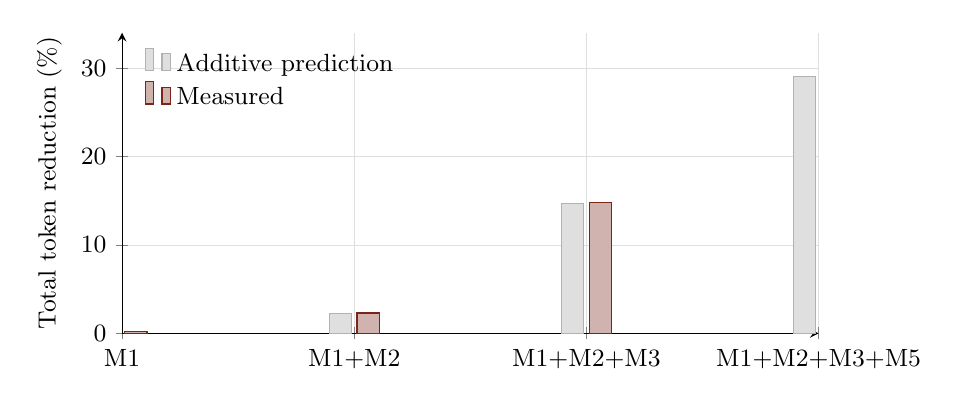
\begin{tikzpicture}
\begin{axis}[
  width=0.86\textwidth, height=5.4cm,
  ybar, bar width=8pt,
  ymin=0, ymax=34,
  ylabel={Total token reduction (\%)},
  ylabel style={font=\small},
  symbolic x coords={M1,M1+M2,M1+M2+M3,M1+M2+M3+M5},
  xtick=data, xticklabel style={font=\small},
  ytick={0,10,20,30},
  tick label style={font=\small},
  legend style={font=\small, at={(0.02,0.97)}, anchor=north west, draw=none,
                fill=none, cells={anchor=west}},
  enlarge x limits=0.18,
  grid=both, grid style={line width=.2pt, draw=gray!25},
  axis lines=left,
]
\addplot+[draw=gray!60, fill=gray!25] coordinates
  {(M1,0.2) (M1+M2,2.2) (M1+M2+M3,14.7) (M1+M2+M3+M5,29.0)};
\addplot+[draw=accent, fill=accent!35] coordinates
  {(M1,0.2) (M1+M2,2.3) (M1+M2+M3,14.8) (M1+M2+M3+M5,27.4)};
\legend{Additive prediction, Measured}
\end{axis}
\end{tikzpicture}
\caption{E1 --- measured reduction against the additive prediction as modules are
accumulated. The two series are indistinguishable until the output budgeter is
added, at which point the measured value falls 1.6\,pp short.}
\label{fig:additivity}
\end{figure}

\begin{table}[htbp]
\centering
\caption{E1 --- estimated effects and effect sizes. All terms of order 3 and
above are $|{\cdot}| < 0.01$\,pp and are omitted.}
\label{tab:effects}
\footnotesize
\begin{tabular}{@{}l l r r@{}}
\toprule
\textbf{Term} & \textbf{Order} & \textbf{Estimate (pp)} & \textbf{Partial $\eta^2$} \\
\midrule
M5 (output budgeter)  & 1 & $+13.43$ & 0.5560 \\
M3 (history manager)  & 1 & $+11.82$ & 0.4308 \\
M2 (semantic cache)   & 1 & $+1.93$  & 0.0115 \\
M1 (compressor)       & 1 & $+0.23$  & 0.0002 \\
\midrule
M3 $\times$ M5        & 2 & \hl{$\mathbf{-0.70}$} & 0.0015 \\
M2 $\times$ M5        & 2 & $-0.11$  & 0.0000 \\
M1 $\times$ M5        & 2 & $-0.02$  & 0.0000 \\
M1 $\times$ M2        & 2 & $+0.02$  & 0.0000 \\
M1 $\times$ M3, M2 $\times$ M3 & 2 & $\pm 0.00$ & 0.0000 \\
\bottomrule
\end{tabular}
\end{table}

\obs{Savings do not compound, and the shortfall is not diffuse --- it is one
term. Of the eleven interaction terms estimated, ten are within $\pm0.11$\,pp of
zero; the entire departure from additivity is carried by $M3\times M5 = -0.70$\,pp,
with $M2\times M5$ contributing a further $-0.11$. Both involve M5, and the
mechanism is visible in the token columns of Table~\ref{tab:ablation}: M3 removes
history from the input while M5 shortens the answer, and in a multi-turn corpus a
shortened answer becomes the next turn's history, so the two modules compete for
the same tokens. The two largest contributors, M5 ($\eta^2=0.556$) and M3
($\eta^2=0.430$), together explain almost all the explained variance, whereas M1
is indistinguishable from zero at $+0.23$\,pp --- a compressor is the technique
with the largest literature and the smallest measured effect here. Finally, the
gap between M1+M2+M3+M5 ($+27.4\%$) and the full stack ($+33.9\%$) is produced
almost entirely by M6a's deterministic routing of 15 requests to zero model
tokens, a component with no compression literature at all.}

\plain{Think of four people cleaning the same room. Alone, they clear 29 bags of
rubbish between them. Working together they clear only 27.4, because two of them
keep reaching for the same rubbish. We found exactly which two: the history
trimmer and the answer shortener. Everything else stacks fine. Also worth
noticing: the compressor --- the trick with the most research papers written about
it --- was the least useful thing we switched on, worth only 0.23\%.}

\subsubsection{Sensitivity across query classes}

The headline percentage conceals a wide per-class spread
(Table~\ref{tab:perclass}).

\begin{table}[htbp]
\centering
\caption{E1 --- token reduction by query class for four representative
configurations.}
\label{tab:perclass}
\footnotesize
\begin{tabular}{@{}l rrrrrr@{}}
\toprule
\textbf{Configuration} & \textbf{Arith.} & \textbf{Code} & \textbf{Factual} &
\textbf{Follow-up} & \textbf{Paraphr.} & \textbf{Summar.} \\
\midrule
M1 only        & \phantom{+}0.0 & +2.8  & +1.1  & \phantom{+}0.0 & $-0.5$ & +0.9 \\
M2 only        & \phantom{+}0.0 & +4.0  & \phantom{+}0.0 & +0.2 & +33.0 & \phantom{+}0.0 \\
M3 only        & \phantom{+}0.0 & \phantom{+}0.0 & \phantom{+}0.0 & +17.3 & \phantom{+}0.0 & \phantom{+}0.0 \\
M1+M2+M3+M5    & +16.8 & +17.6 & +13.6 & +30.3 & +42.5 & +12.0 \\
\textbf{Full stack} & \hl{\textbf{+69.3}} & +30.8 & +22.8 & +32.4 & +49.2 & +20.7 \\
\bottomrule
\end{tabular}
\end{table}

\obs{No module is uniformly useful. M3 delivers $+17.3$\,pp on follow-up queries
and exactly zero on the other five classes, because only follow-ups carry history
worth trimming. M2 delivers $+33.0$\,pp on paraphrases and near-zero elsewhere,
which is what a cache should do. The full stack's $+69.3$\,pp on arithmetic is
M6a answering without the model at all. This spread is the empirical argument for
the paper's central claim that the deliverable is an operating curve rather than
a number: a deployment serving mostly summarisation should expect 20\%, not 34\%.
The one apparently negative entry, M1 at $-0.5$\,pp on paraphrases, is an
artefact and not a regression; §\ref{sec:artefact} separates it out.}

\plain{The ``33.9\% saving'' is an average, and averages hide a lot. If your
users mostly ask maths questions you save 69\%; if they mostly ask for summaries
you save 21\%. That is why we say the real result of this project is not a number
but a recipe --- ``for your kind of traffic, switch on these parts''.}

\subsubsection{Separating a measurement artefact from a regression}
\label{sec:artefact}

One cell of Table~\ref{tab:perclass} shows a saving below zero: M1 on paraphrase
traffic, $-0.5$\,pp. Because the combined column cannot say whether a module
acted on the prompt or on the answer, that entry was re-measured with input and
output separated.

\begin{table}[htbp]
\centering
\caption{E1 --- M1 against baseline, input and output tokens separated, by query
class. The combined column is the sum of the two and is what
Table~\ref{tab:perclass} reports.}
\label{tab:m1split}
\footnotesize
\begin{tabular}{@{}l rr r rr r r@{}}
\toprule
& \multicolumn{2}{c}{\textbf{Input tokens}} & &
  \multicolumn{2}{c}{\textbf{Output tokens}} & & \\
\cmidrule(lr){2-3}\cmidrule(lr){5-6}
\textbf{Class} & \textbf{Base} & \textbf{M1} & $\boldsymbol{\Delta}$ &
\textbf{Base} & \textbf{M1} & $\boldsymbol{\Delta}$ & \textbf{Combined} \\
\midrule
arithmetic    &   929 &   929 & \phantom{$-$}0 & 1{,}782 & 1{,}782 & \phantom{$-$}0 & \phantom{$+$}0.00 \\
code          &   947 &   934 & $-13$ & 1{,}699 & 1{,}639 & $-60$ & $+2.76$ \\
factual       &   791 &   768 & $-23$ & 1{,}546 & 1{,}544 & $-2$  & $+1.07$ \\
follow\_up    & 26{,}901 & 26{,}901 & \phantom{$-$}0 & 8{,}706 & 8{,}706 & \phantom{$-$}0 & \phantom{$+$}0.00 \\
paraphrase    &   755 &   743 & $\mathbf{-12}$ & 1{,}725 & 1{,}749 & $\mathbf{+24}$ & $\mathbf{-0.48}$ \\
summarisation & 1{,}637 & 1{,}613 & $-24$ & 1{,}744 & 1{,}739 & $-5$  & $+0.86$ \\
\bottomrule
\end{tabular}
\end{table}

\obs{The negative entry is entirely output-side, and it is a property of the
provider rather than of compression. On paraphrase queries M1 \emph{did} shorten
the prompt, by 12 tokens; the response then grew by 24. The deterministic
provider's output length is a function of the prompt it is given, so any module
that changes the prompt perturbs the answer length in a direction that carries no
meaning --- and M2 is switched off in this cell, so no cache hit can have been
lost. An explanation in terms of the compression--cache interaction of Gap 3,
which the combined column invites, is therefore unavailable: the mechanism it
names is not present in the configuration being measured. The general lesson is
that a combined token figure can attribute a provider artefact to a module. Input
reduction is the quantity that survives this objection, because it is counted
with the model's own tokenizer before generation happens, and it is also the
quantity that converts into prefill time. Movements below roughly 1\% in the
output column should be read as zero.}

\subsubsection{Where compression actually pays}

\begin{table}[htbp]
\centering
\caption{E1 --- outcome of every edit M1 proposed, by edit regime.}
\label{tab:tokenprobe}
\footnotesize
\begin{tabular}{@{}l rrrr r@{}}
\toprule
\textbf{Edit regime} & \textbf{Tested} & \textbf{Saved} & \textbf{Saved nothing} &
\textbf{Cost tokens} & \textbf{Wasted (\%)} \\
\midrule
Phrase-level    & 21    & 21    & 0  & 0 & 0 \\
Word-level      & 2{,}199 & 2{,}183 & 13 & 3 & 1 \\
Sub-token-level & 8     & 0     & 5  & 3 & \hl{\textbf{100}} \\
\bottomrule
\end{tabular}
\end{table}

\obs{Whitespace-aligned edits are effectively monotone, and sub-token edits are
never worth making. Of 2{,}199 word deletions, 2{,}183 reduced the token count and
only 3 increased it, because modern byte-pair encoders attach the leading space to
the following token, so removing a whole word removes whole tokens. Every one of
the 8 sub-token edits failed --- 5 saved nothing and 3 actively increased the count.
This localises the ``negative yield'' phenomenon the compression literature warns
about: it is not a property of compression in general but of edits that cut
\emph{inside} a token boundary, and a guard that measures the resulting count
rather than assuming a reduction eliminates the class entirely.}

\plain{Deleting a \emph{whole word} almost always makes the prompt cheaper ---
2{,}183 times out of 2{,}199. But cutting \emph{inside} a word is never worth it:
all 8 attempts failed, and 3 of them made the prompt \emph{longer}. So the
warning in the literature that ``shortening text can cost you tokens'' is true,
but only for one specific kind of edit, and our guard simply checks the count
afterwards instead of trusting the edit.}

\subsection{E2: What does a token cost, and what does prompt order cost?}
\label{sec:e2}

\textbf{Baseline:} for the split measurement, none --- this is a characterisation.
For the arrangement measurement, a prompt whose head carries a volatile token.
\textbf{Proposed:} M4's arrangement, invariant content first.
\textbf{Instrument:} the server's own \texttt{prompt\_eval\_duration} and
\texttt{eval\_duration} counters rather than wall-clock time-to-first-token,
which conflates queueing and sampling with prefill.

\begin{table}[htbp]
\centering
\caption{E2 --- prefill/decode split against \texttt{qwen2.5:1.5b-instruct}
(Q4\_K\_M) on CPU.}
\label{tab:prefill}
\footnotesize
\begin{tabular}{@{}r rr r r@{}}
\toprule
\textbf{Input tokens} & \textbf{Prefill (ms)} & \textbf{Decode (ms)} &
\textbf{Prefill share (\%)} & \textbf{ms / input token} \\
\midrule
146    & 1{,}360  & 122 & 91.7 & 9.3 \\
474    & 3{,}902  & 165 & 95.9 & 8.2 \\
1{,}338 & 11{,}609 & 136 & \hl{98.8} & 8.7 \\
\bottomrule
\end{tabular}
\end{table}

\begin{table}[htbp]
\centering
\caption{E2 --- steady-state cost of two prompt arrangements carrying the same
content.}
\label{tab:prefix}
\footnotesize
\begin{tabular}{@{}l r r r@{}}
\toprule
\textbf{Arrangement} & \textbf{Tokens} & \textbf{Steady-state prefill (ms)} &
\textbf{Prefix reuse (\%)} \\
\midrule
Volatile head (baseline)   & 1{,}497 & 18{,}914 & 0.5 \\
Stable prefix (M4)         & 1{,}490 & \hl{\textbf{212}} & \textbf{98.5} \\
\midrule
\textbf{Difference}        & $-0.5\%$ & $\mathbf{-98.9\%}$ & $+98.0$\,pp \\
\bottomrule
\end{tabular}
\end{table}

\obs{Prefill dominates, and the dominance strengthens with context length ---
91.7\% at 146 input tokens rising to 98.8\% at 1{,}338. The per-token cost is
essentially constant at 8.2--9.3\,ms, so prefill is linear in input length and
input reduction converts directly into wall-clock time: the 11{,}836 input tokens
the full stack removes are $\approx$100.6\,s of prefill across the corpus, or
383\,ms per request. This refutes the premise stated in Gap 2, which anticipated
that sequential decode would dominate on CPU; the measurement says the opposite,
and the correct conclusion is that the literature's input-side focus is right for
the wrong reason. Table~\ref{tab:prefix} then shows that a token counter is an
unreliable proxy for cost: two prompts 0.5\% apart in tokens differ by
$\approx$89$\times$ in steady-state prefill, because one preserves the key-value
cache and the other invalidates it every turn. Any optimiser that reorders a
prompt to place relevant content first --- the remedy \emph{recommended} by [28]
--- pays this cost, and every token-based metric in the compression literature
scores the two arrangements identically.}

\plain{Almost all the waiting is the model \emph{reading} your question, not
writing the reply --- and the longer the conversation, the more lopsided it gets.
Every input token costs about 8.5 milliseconds, so cutting words really does cut
seconds: across our whole test set the system saved about 100 seconds of reading.
The surprise is the second table. The model keeps a memory of the prompt it just
read, and it can skip anything at the start that has not changed. Put something
that changes every turn at the very beginning and that memory is thrown away
every time. Two prompts with virtually the same number of words: one takes a
fifth of a second, the other takes nineteen seconds. A word counter cannot see
this difference at all --- which is the point.}

\subsection{E3: Can a threshold make cache reuse safe?}
\label{sec:e3}

\textbf{Baseline:} threshold-only cache, verifier disabled --- the design used by
[16] and every system that follows it.
\textbf{Proposed:} the same cache with a four-check invariant verifier over
numbers, named entities, negations and operative modifiers.
\textbf{Variable:} the acceptance threshold $\tau$, swept over nine values.
\textbf{Hypothesis tested:} that some $\tau$ separates genuine paraphrases from
one-token meaning inversions.

\begin{table}[htbp]
\centering
\caption{E3 --- threshold sweep over 45 adversarial pairs and 45 controls.}
\label{tab:calib}
\footnotesize
\begin{tabular}{@{}l rr rr@{}}
\toprule
& \multicolumn{2}{c}{\textbf{Verifier off (baseline)}} &
  \multicolumn{2}{c}{\textbf{Verifier on (proposed)}} \\
\cmidrule(lr){2-3}\cmidrule(lr){4-5}
$\boldsymbol{\tau}$ & \textbf{False hits} & \textbf{True hits} &
                      \textbf{False hits} & \textbf{True hits} \\
\midrule
0.70 & 31/45 (68.9\%) & 25/45 (55.6\%) & 31/45 (68.9\%) & 25/45 (55.6\%) \\
0.75 & 23/45 (51.1\%) & 18/45 (40.0\%) & 23/45 (51.1\%) & 18/45 (40.0\%) \\
0.80 & 23/45 (51.1\%) & 18/45 (40.0\%) & 17/45 (37.8\%) & 17/45 (37.8\%) \\
0.85 & 23/45 (51.1\%) & 18/45 (40.0\%) & \phantom{0}8/45 (17.8\%) & 17/45 (37.8\%) \\
0.90 & 23/45 (51.1\%) & 18/45 (40.0\%) & \phantom{0}2/45 (4.4\%) & 16/45 (35.6\%) \\
\textbf{0.92} & 23/45 (51.1\%) & 18/45 (40.0\%) & \hl{\textbf{0/45 (0.0\%)}} & \textbf{14/45 (31.1\%)} \\
0.95 & 23/45 (51.1\%) & 18/45 (40.0\%) & 0/45 (0.0\%) & 13/45 (28.9\%) \\
0.97 & 23/45 (51.1\%) & 18/45 (40.0\%) & 0/45 (0.0\%) & 13/45 (28.9\%) \\
0.99 & 23/45 (51.1\%) & 18/45 (40.0\%) & 0/45 (0.0\%) & 13/45 (28.9\%) \\
\bottomrule
\end{tabular}
\end{table}

\begin{figure}[htbp]
\centering
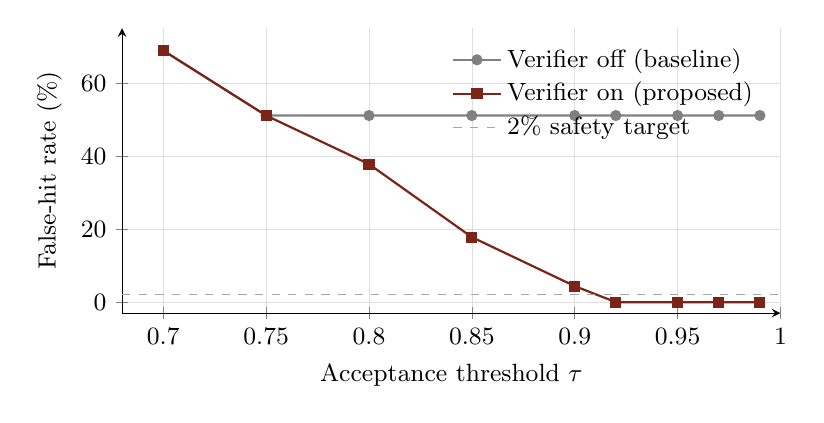
\begin{tikzpicture}
\begin{axis}[
  width=0.82\textwidth, height=5.2cm,
  xlabel={Acceptance threshold $\tau$}, ylabel={False-hit rate (\%)},
  xlabel style={font=\small}, ylabel style={font=\small},
  tick label style={font=\small},
  xmin=0.68, xmax=1.0, ymin=-3, ymax=75,
  legend style={font=\small, at={(0.98,0.97)}, anchor=north east, draw=none,
                fill=none, cells={anchor=west}},
  grid=both, grid style={line width=.2pt, draw=gray!25}, axis lines=left,
]
\addplot[thick, mark=*, mark size=1.6pt, gray] coordinates
  {(0.70,68.9) (0.75,51.1) (0.80,51.1) (0.85,51.1) (0.90,51.1)
   (0.92,51.1) (0.95,51.1) (0.97,51.1) (0.99,51.1)};
\addplot[thick, mark=square*, mark size=1.6pt, accent] coordinates
  {(0.70,68.9) (0.75,51.1) (0.80,37.8) (0.85,17.8) (0.90,4.4)
   (0.92,0.0) (0.95,0.0) (0.97,0.0) (0.99,0.0)};
\addplot[dashed, gray!70, thin] coordinates {(0.68,2) (1.0,2)};
\legend{Verifier off (baseline), Verifier on (proposed), 2\% safety target}
\end{axis}
\end{tikzpicture}
\caption{E3 --- false-hit rate against acceptance threshold. Raising the
threshold alone does not help beyond $\tau = 0.75$; the baseline curve is flat at
51.1\% all the way to $\tau = 0.99$.}
\label{fig:threshold}
\end{figure}

\begin{table}[htbp]
\centering
\caption{E3 --- residual false hits by the operative token that distinguishes the
pair, at the deployed operating point $\tau = 0.92$ with the verifier enabled.}
\label{tab:operative}
\footnotesize
\begin{tabular}{@{}l r r@{}}
\toprule
\textbf{Distinguishing token} & \textbf{False hits} & \textbf{Rate (\%)} \\
\midrule
Number              & 0/14 & 0.0 \\
Negation            & 0/13 & 0.0 \\
Named entity        & 0/9  & 0.0 \\
Operative modifier  & 0/9  & 0.0 \\
\midrule
\textbf{Overall}    & \textbf{0/45} & \textbf{0.0} \\
\bottomrule
\end{tabular}
\end{table}

\obs{The hypothesis is refuted decisively: \emph{no threshold is safe}. The
verifier-off curve is flat at 51.1\% from $\tau=0.75$ to $\tau=0.99$ --- pushing
the threshold to 0.99 rejects genuine paraphrases without rejecting a single
additional adversarial pair, because the adversarial pairs sit \emph{above} the
paraphrases in similarity. A one-token negation is a smaller edit in embedding
space than a full rewording, so the ordering the threshold relies on is inverted
for exactly the cases where being wrong is most costly. The published safe range
of 0.85--0.92 sits squarely inside the flat region and would serve the opposite
answer in roughly half of adversarial cases. The verifier changes the shape of the
curve rather than shifting it, reaching 0/45 at $\tau = 0.92$ and holding there,
and Table~\ref{tab:operative} shows the residual is zero in all four operative
categories rather than concentrated in an easy one. The cost is a true-hit rate of
31.1\% against the baseline's 40.0\%: \textbf{8.9\,pp of genuine reuse is
surrendered to eliminate 51.1\,pp of wrong answers}, which is the central
efficiency--safety trade-off of this system and, for an assistant, plainly the
right side of it.}

\plain{Every cache in the research literature works the same way: if the new
question is ``similar enough'' to an old one, reuse the old answer. We tested
whether \emph{any} setting of ``similar enough'' is safe. It is not. We tried
nine settings from loose to extremely strict, and the error rate never moved
below 51\% --- because ``Is it safe?'' and ``Is it \emph{not} safe?'' are almost
identical to a computer, while two genuinely different wordings of the same
question look far apart. So the strictest setting throws away good matches
without catching a single bad one. Our fix does not compare meaning at all: it
just lists the numbers, names, ``not''s and words like ``cheapest'' in both
questions and refuses if they differ. That takes microseconds and got the errors
to zero. The price is that we now miss about 9 out of every 100 reuses we could
have had --- worth paying, since the alternative is confidently telling someone
that mixing bleach and vinegar is safe.}

\subsection{E4: Is quality preserved, and at what overhead?}
\label{sec:e4}

\textbf{Baseline:} unoptimised pipeline, real model.
\textbf{Proposed:} full stack, real model.
\textbf{Design:} paired per item over the 40-item gold subset, so that an
improvement and a regression cannot cancel in the aggregate.

\begin{table}[htbp]
\centering
\caption{E4 --- answer quality on the 40-item gold subset against the real model.}
\label{tab:quality}
\footnotesize
\begin{tabular}{@{}l r r r@{}}
\toprule
\textbf{Configuration} & \textbf{Gold correct} & \textbf{Accuracy (\%)} &
\textbf{Regressions} \\
\midrule
Baseline    & 37/40 & 92.5 & --- \\
Full stack  & \textbf{39/40} & \hl{\textbf{97.5}} & \hl{\textbf{0}} \\
\bottomrule
\end{tabular}
\end{table}

\begin{table}[htbp]
\centering
\caption{E4 --- middleware overhead per request, model time excluded, over 263
requests.}
\label{tab:overhead}
\footnotesize
\begin{tabular}{@{}l r l r r@{}}
\toprule
\textbf{Configuration} & \textbf{Mean (ms)} & \textbf{95\% CI} &
\textbf{p95 (ms)} & \textbf{Prefix tokens reused} \\
\midrule
Baseline (all off)   & 2.01 & [1.80, 2.24] & 4.81 & 1.4 \\
M2 only              & 2.74 & [2.53, 2.94] & 5.65 & 1.4 \\
M1+M2+M3             & 3.62 & [3.30, 3.91] & 7.15 & 1.4 \\
M1+M2+M3+M5          & 3.60 & [3.32, 3.89] & 6.92 & 1.4 \\
\textbf{Full stack}  & \hl{\textbf{4.06}} & \textbf{[3.68, 4.45]} & \textbf{9.49} &
\textbf{14.1} \\
\midrule
\multicolumn{5}{@{}l}{\textit{Design budget: 120\,ms}} \\
\bottomrule
\end{tabular}
\end{table}

\obs{The optimisation is not paid for in quality or in overhead. Accuracy moves
from 37/40 to 39/40, and the paired analysis shows \textbf{zero regressions}: no
item the baseline answered correctly was lost, so the two-item gain is not
masking offsetting damage. The gains are arithmetic items routed to M6a and
answered exactly without the model, and two discordant pairs is not statistically
significant (exact McNemar, $p = 0.50$); the defensible claim is therefore
\emph{no measurable degradation}, not improvement. On cost, the full stack adds
2.05\,ms over baseline for a mean of 4.06\,ms, roughly 30$\times$ inside the
120\,ms design budget and approximately 0.24\% of the $\approx$1.7\,s the same
request spends in prefill at typical context length --- so the stack pays for
itself by a factor of several hundred. The prefix-reuse column isolates M4's
contribution: reuse rises from 1.4 tokens to 14.1 only in the configuration where
M4 is enabled, confirming that no other module preserves the prompt head by
accident.}

\plain{This is the section that answers ``yes, but does it break anything?''
Answer: no. Out of 40 test questions the plain system got 37 right and ours got
39 --- and crucially, we checked question by question, so we know ours did not
quietly get something wrong that the plain system got right. Not once. The two
extra correct answers are sums that our system worked out itself without
bothering the model. Two questions is too few to claim we made it \emph{smarter},
so we only claim we did not make it worse. On speed, our own code adds about 4
thousandths of a second per question --- next to the roughly 1.7 seconds the model
spends reading, that is nothing.}

\subsection{E5: Does a calibration transfer?}
\label{sec:e5}

\textbf{Baseline (5a):} thresholds and module settings calibrated on Qwen2.5's
151{,}665-entry vocabulary. \textbf{Proposed:} the identical protocol re-run
under GPT-2's 50{,}257-entry vocabulary with \emph{no} re-tuning.
\textbf{Baseline (5b):} a cold cache. \textbf{Proposed:} a cache warm-started
from a disjoint half of the conversations, evaluated on the held-out half.

\begin{table}[htbp]
\centering
\caption{E5a --- per-module reduction replicated under a second tokenizer
vocabulary with settings carried over unchanged.}
\label{tab:generalisation}
\footnotesize
\begin{tabular}{@{}l r r r@{}}
\toprule
\textbf{Configuration} & \textbf{Qwen2.5 (151{,}665)} & \textbf{GPT-2 (50{,}257)} &
\textbf{Difference (pp)} \\
\midrule
M1 only        & +0.23  & +0.22  & 0.01 \\
M2 only        & +2.03  & +2.04  & 0.01 \\
M3 only        & +12.52 & +12.61 & 0.09 \\
M5 only        & +14.27 & +14.24 & 0.03 \\
M1+M2+M3+M5    & +27.43 & +27.35 & 0.08 \\
\bottomrule
\end{tabular}
\end{table}

\begin{table}[htbp]
\centering
\caption{E5a --- transfer of the tokenizer-level \emph{explanations} offered for
those reductions.}
\label{tab:claims}
\footnotesize
\begin{tabularx}{\textwidth}{@{}X l l c@{}}
\toprule
\textbf{Claim under test} & \textbf{Qwen2.5} & \textbf{GPT-2} & \textbf{Transfers} \\
\midrule
Leading-space form is cheaper (`` happened'' vs ``happened'') & 1 vs 3 & 1 vs 3 & yes \\
Capitalisation costs a token (``explain'' vs ``Explain'')     & 1 vs 2 & 2 vs 2 & \textbf{no} \\
First-word deletion can raise the count                        & 11 vs 12 & 7 vs 8 & yes \\
Tier-1 normalisations that save nothing                        & 7/20 (35\%) & 7/20 (35\%) & yes \\
\bottomrule
\end{tabularx}
\end{table}

\begin{table}[htbp]
\centering
\caption{E5b --- warm-start benefit on held-out conversations as a function of
traffic recurrence.}
\label{tab:learning}
\footnotesize
\begin{tabular}{@{}r r rr r r@{}}
\toprule
\textbf{Recurrence (\%)} & \textbf{Cache seeds} & \textbf{Cold (\%)} &
\textbf{Warm (\%)} & \textbf{Transfer (pp)} & \textbf{Extra gate fires} \\
\midrule
0.0  & 0  & 8.20  & 8.20  & \hl{\textbf{+0.00}} & 0 \\
7.5  & 3  & 12.16 & 13.48 & +1.31  & 0 \\
22.5 & 8  & 15.76 & 21.19 & +5.43  & 0 \\
33.3 & 10 & 24.21 & 32.76 & +8.55  & 0 \\
45.0 & 12 & 34.16 & 48.87 & +14.70 & 0 \\
57.5 & 16 & 45.69 & 63.52 & \hl{\textbf{+17.83}} & 0 \\
\bottomrule
\end{tabular}
\end{table}

\begin{figure}[htbp]
\centering
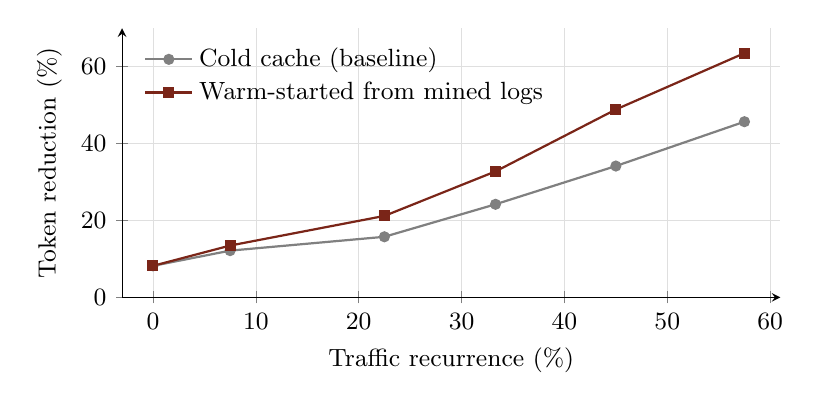
\begin{tikzpicture}
\begin{axis}[
  width=0.82\textwidth, height=5.0cm,
  xlabel={Traffic recurrence (\%)}, ylabel={Token reduction (\%)},
  xlabel style={font=\small}, ylabel style={font=\small},
  tick label style={font=\small},
  xmin=-3, xmax=61, ymin=0, ymax=70,
  legend style={font=\small, at={(0.02,0.97)}, anchor=north west, draw=none,
                fill=none, cells={anchor=west}},
  grid=both, grid style={line width=.2pt, draw=gray!25}, axis lines=left,
]
\addplot[thick, mark=*, mark size=1.6pt, gray] coordinates
  {(0,8.20) (7.5,12.16) (22.5,15.76) (33.3,24.21) (45,34.16) (57.5,45.69)};
\addplot[thick, mark=square*, mark size=1.6pt, accent] coordinates
  {(0,8.20) (7.5,13.48) (22.5,21.19) (33.3,32.76) (45,48.87) (57.5,63.52)};
\legend{Cold cache (baseline), Warm-started from mined logs}
\end{axis}
\end{tikzpicture}
\caption{E5b --- warm-start benefit against traffic recurrence, measured on
conversations disjoint from those mined. The curves meet exactly at zero
recurrence.}
\label{fig:learning}
\end{figure}

\obs{A calibration transfers as a \emph{ratio} but not as a \emph{mechanism}.
Every per-module reduction replicates under a vocabulary three times smaller to
within 0.09\,pp with the module ranking unchanged (Table~\ref{tab:generalisation}),
because a reduction percentage cancels a roughly constant vocabulary factor. The
explanations fare worse: one of the four tokenizer-level claims we ourselves
advanced --- that capitalisation costs a token --- is false under GPT-2, which
charges two tokens either way (Table~\ref{tab:claims}). Half of one stated
mechanism was a Qwen-specific fact presented as a general one, and only
replication exposed it. On the second axis, Table~\ref{tab:learning} makes
``self-improving'' measurable rather than rhetorical: the benefit is
\emph{monotone in recurrence} and is \textbf{exactly $+0.00$\,pp at 0\%
recurrence}, which is the result that makes the remainder credible --- a mining
procedure that leaked would have shown a spurious gain there. The evaluation
corpus itself sits at 1.9\% recurrence, which is why M7 contributes nothing to
Table~\ref{tab:ablation}; that is a property of the corpus, not of the module. In
all six conditions the fidelity gate fired zero additional times, so the extra
reuse is not being bought with extra risk.}

\plain{Two questions here. First: tune the system for one model's vocabulary ---
does it still work for another? The \emph{savings} carried over almost perfectly,
within a tenth of a percent. But one of our own explanations for \emph{why} it
saves turned out to be wrong on the second vocabulary. That is worth saying out
loud: we were half wrong about our own system, and only re-running the test caught
it. Second: the system learns from your past chats to pre-fill its memory. Does
that help on chats it has never seen? It depends entirely on how much you repeat
yourself. If you never repeat a question the benefit is \emph{exactly} zero --- and
that exact zero is the most important number in the table, because a system that
was secretly peeking at the test data would have shown a fake gain there. The more
you repeat, the more it helps, up to about 18\% extra saving.}

\subsection{Contribution-to-result summary}
\label{sec:summary}

\begin{table}[htbp]
\centering
\caption{Contribution, question, evidence and finding.}
\label{tab:summary}
\scriptsize
\begin{tabularx}{\textwidth}{@{}l c c L{2.6cm} X@{}}
\toprule
& \textbf{RQ} & \textbf{Exp.} & \textbf{Evidence} & \textbf{Finding} \\
\midrule
C1 & RQ1 & E1 & Tables~\ref{tab:ablation}, \ref{tab:effects}; Fig.~\ref{fig:additivity} &
  Savings are not additive: 29.0\,pp predicted, 27.4\,pp measured. The 1.66\,pp shortfall is carried almost entirely by one negative interaction, $M3\times M5 = -0.70$\,pp. \\
\addlinespace
C2 & RQ2 & E2 & Tables~\ref{tab:prefill}, \ref{tab:prefix} &
  Prefill is 91.7--98.8\% of inference time at $\approx$8.5\,ms/token. Two prompts 0.5\% apart in tokens differ $\approx$89$\times$ in cost, so token count is not a reliable proxy for cost on CPU. \\
\addlinespace
C3 & RQ3 & E3 & Table~\ref{tab:calib}; Fig.~\ref{fig:threshold} &
  No threshold is safe: the false-hit rate is flat at 51.1\% from $\tau=0.75$ to $0.99$. A four-check verifier reaches 0/45 at $\tau=0.92$, surrendering 8.9\,pp of true hits. \\
\addlinespace
C4 & RQ4 & E4 & Tables~\ref{tab:quality}, \ref{tab:overhead} &
  92.5\% $\rightarrow$ 97.5\% gold accuracy with zero paired regressions, at 4.06\,ms mean middleware overhead --- roughly 30$\times$ inside the design budget. \\
\addlinespace
C5 & RQ5 & E5 & Tables~\ref{tab:generalisation}--\ref{tab:learning}; Fig.~\ref{fig:learning} &
  Reduction ratios replicate across vocabularies within 0.09\,pp, but one of four stated mechanisms does not. Warm-start transfer is monotone in recurrence, exactly $+0.00$\,pp at 0\%. \\
\bottomrule
\end{tabularx}
\end{table}

% ================================================ 6 DISCUSSION =========
\section{Discussion}
\label{sec:discussion}

The previous section reported \emph{what} happened. This section argues about
\emph{why}, and is careful to separate the two: measurements are stated as
results, explanations as explanations.

\subsection{Why the savings fail to compound}
The shortfall is not a general property of stacking but the signature of two
modules addressing the same tokens. M3 removes prior turns from the input; M5
shortens the generated answer. In a multi-turn conversation the answer M5 shortens
becomes part of the history M3 will later trim, so the second module to act finds
less material than it would have found alone. This explains both the sign and the
localisation: the interaction is negative, and it appears only in terms containing
M5. It also predicts the boundary condition --- in single-turn traffic the two
modules should be additive, because no answer ever becomes history. That
prediction is untested here and is stated as a hypothesis, not a result.

\plain{Today's answer becomes tomorrow's chat history. So when one part of the
system shortens the answer, it is also shrinking the pile that the other part was
going to trim later. Whichever runs second finds less left to do. That neatly
explains why the overlap only ever shows up between those two parts. It also
gives us something to check next: in a one-question-at-a-time chat, where an
answer never becomes history, the two should stop overlapping. We have not tested
that, so we call it a prediction rather than a finding.}

\subsection{Why a threshold cannot separate the classes}
The flat baseline curve in Figure~\ref{fig:threshold} follows from what
sentence-level similarity measures. Inserting ``not'' changes one token in twelve
and leaves topic, entities and syntax intact, whereas a genuine paraphrase may
replace most content words. Similarity ranks the adversarial pair above the
paraphrase, so the ordering a threshold relies upon is inverted precisely where
the consequences are worst. Any monotone function of that similarity inherits the
inversion, which is why the fix has to inspect the tokens that carry the meaning
rather than the geometry. Our conclusion agrees with [22], which reaches it by a
different route; the contribution here is that four set comparisons costing
microseconds suffice, so safety need not be bought with a second model.

\subsection{Agreement and disagreement with prior work}
The finding that input reduction is what matters agrees with the compression
literature's emphasis, but for a different reason than that literature gives:
not because the prompt is what is billed, but because prefill is what is slow.
The disagreement is sharper for [28]. Placing relevant content at the prompt head
is sound advice for attention and, on this hardware, catastrophic for cost. The
two results are not contradictory --- they optimise different quantities --- but no
paper in either strand prices the exchange, and Table~\ref{tab:prefix} suggests
the exchange rate is unfavourable by roughly two orders of magnitude. Finally,
routing assumptions from the cascade literature [32], [33] do not survive the
descent in scale: a 3B model scored 36/40 against the 1.5B model's 36/40 on our
gold subset, item for item, so M6's escalation tier is calibrated but disabled.

\subsection{What the results imply for deployment}
Three implications follow. First, module selection should be conditioned on query
mix: Table~\ref{tab:perclass} shows a 3.4$\times$ spread in benefit across
classes, and M1 earns its place on code and summarisation traffic while
contributing nothing measurable on arithmetic or follow-ups. Second,
the cache verifier should be treated as mandatory rather than as a refinement,
since the alternative is a documented 51.1\% error rate on the adversarial class.
Third, prompt assembly deserves the same engineering attention as compression:
M4 contributes almost nothing to the token metric and more to wall-clock time than
every other module combined.

% ================================================ 7 LIMITATIONS =======
\section{Limitations and Threats to Validity}
\label{sec:limits}

\plain{This section lists what our results do \emph{not} prove, and what we did
not manage to measure. Everything marked \texttt{[MEASUREMENT REQUIRED]} is an
experiment still to be run --- we have deliberately left the gap visible rather
than filling it with a guessed number.}

\paragraph{Single hardware configuration.} All timings come from one CPU. The
8.5\,ms per input token figure is a measurement of this machine, not a claim
about CPUs generally; the qualitative finding that prefill dominates is expected
to be more robust than the coefficient.

\paragraph{Simulated provider in three experiments.} E1, E3 and E5 run against a
deterministic provider for exact reproducibility. Token counts there are real,
computed with the deployed tokenizer, but the \emph{answers} are not model
outputs, so those experiments measure token economics rather than answer quality.
E4 supplies the real-model quality evidence and covers only the baseline-vs-full-
stack contrast. Per-configuration quality on the real model is not established:
\todoval{gold accuracy for each of the 17 configurations, real model, paired per
item}

\paragraph{The provider's output length responds to the prompt.} In E1, E3 and E5
the answer length is a function of the prompt, so any module that edits the
prompt perturbs the output token count in a direction that carries no meaning.
The effect is small --- at most 24 tokens in a single class-cell
(Table~\ref{tab:m1split}) --- but it is large enough to move a per-class combined
figure across zero, and it is why every reduction in this paper is also reported
on input tokens alone (Table~\ref{tab:inputside}). Output-side movements below
about 1\% should be read as zero. The input-side figures are unaffected: they are
tokenizer counts taken before generation.

\paragraph{Small gold subset.} Forty items is enough to demonstrate the absence of
regressions but not to resolve small differences; the McNemar test on two
discordant pairs is unpowered, which is why no improvement is claimed.

\paragraph{Energy is not measured.} The implemented estimator infers joules from
token throughput and is degenerate: it attributes 0.0\,J to one configuration and
reports the full stack as 39\% \emph{worse} than baseline, which contradicts the
directly measured prefill reduction. No energy result is claimed anywhere in this
paper. A defensible measurement requires socket-level or RAPL instrumentation:
\todoval{joules per request, baseline vs full stack, hardware power counters,
$n \geq 30$ repetitions per configuration}

\paragraph{Memory and CPU utilisation were not instrumented.}
\todoval{peak resident set size and mean CPU utilisation, baseline vs full stack}

\paragraph{Corpus recurrence is 1.9\%.} The evaluation corpus was authored for
ablation diversity, so M7's contribution to Table~\ref{tab:ablation} is
approximately zero. E5b therefore reports a curve over synthetic recurrence
levels rather than a single deployment number. The repetition structure is
synthetic; every question and answer within it is real.

\paragraph{Uncalibrated automatic judge.} A pairwise LLM judge reached 98\%
disagreement between runs on identical inputs and its scores are excluded.
Quality conclusions rest on gold exact match, with embedding similarity and token
overlap as secondary evidence.

\paragraph{Lexical encoder.} The default encoder is lexical rather than neural.
Operating points --- in particular $\tau$ --- shift with the encoder; the module
ranking in Table~\ref{tab:effects} was stable across the two encoders tested.

% ================================================ 8 CONCLUSION ========
\section{Conclusion}
\label{sec:conclusion}

This work composed eight token-optimisation techniques in a single instrumented
pipeline and measured what happens, rather than assuming it. Over 151
conversations and 263 requests the full stack removed 33.9\% of tokens at a mean
middleware cost of 4.06\,ms and with zero paired quality regressions on the gold
subset.

Three results are of independent interest. Savings are not additive, and the
departure is not diffuse but concentrated in a single interaction between the
history manager and the output budgeter, which compete for the same tokens in
multi-turn traffic. On CPU-only hardware, prefill accounts for 91.7--98.8\% of
inference time, which makes token count a good target and a poor proxy: two
prompts 0.5\% apart in tokens can differ by two orders of magnitude in cost,
depending only on whether the prompt head stayed byte-stable. And no similarity
threshold makes cached-answer reuse safe --- the false-hit rate is flat at 51.1\%
across the entire usable range --- whereas four non-neural set comparisons reduce
it to zero at a cost of 8.9\,pp of genuine reuse.

The recurring pattern across all five experiments is that published operating
points are properties of the configuration they were calibrated on. A threshold
described as safe is unsafe here; a placement rule justified by a well-cited
attention result is roughly 89$\times$ more expensive here; a calibration
transfers as a ratio but not as an explanation; a routing premise that holds at
large scale does not hold at 1.5B against 3B. The results indicate that for this
class of system the useful deliverable is a calibration procedure and an operating
curve, not a headline percentage.

Immediate future work is bounded by Section~\ref{sec:limits}: instrumented energy
measurement, per-configuration quality against the real model, and replication of
the prefill coefficient on a second CPU.

% ================================================ REFERENCES ==========
\begin{thebibliography}{40}
\footnotesize
\bibitem{r1} Li, Y., Dong, B., Lin, C., Guerin, F. \emph{Compressing Context to Enhance Inference Efficiency of Large Language Models.} EMNLP, 2023. arXiv:2310.06201.
\bibitem{r2} Jiang, H., Wu, Q., Lin, C.-Y., Yang, Y., Qiu, L. \emph{LLMLingua: Compressing Prompts for Accelerated Inference of Large Language Models.} EMNLP, 2023. arXiv:2310.05736.
\bibitem{r3} Jiang, H., et al. \emph{LongLLMLingua: Accelerating and Enhancing LLMs in Long Context Scenarios via Prompt Compression.} arXiv:2310.06839.
\bibitem{r4} \emph{LLMLingua-2: Data Distillation for Efficient and Faithful Task-Agnostic Prompt Compression.} arXiv:2403.12968.
\bibitem{r5} \emph{Efficient Prompt Compression with Evaluator Heads for Long-Context Transformer Inference.} arXiv:2501.12959.
\bibitem{r6} \emph{SCOPE: A Generative Approach for LLM Prompt Compression.} arXiv:2508.15813.
\bibitem{r7} \emph{Long Context In-Context Compression by Getting to the Gist of Gisting.} arXiv:2504.08934.
\bibitem{r8} \emph{Compressing Lengthy Context With UltraGist.} arXiv:2405.16635.
\bibitem{r9} \emph{ATACompressor: Adaptive Task-Aware Compression for Efficient Long-Context Processing in LLMs.} arXiv:2602.03226.
\bibitem{r10} \emph{SARA: Selective and Adaptive Retrieval-augmented Generation with Context Compression.} arXiv:2507.05633.
\bibitem{r11} \emph{PCToolkit: A Unified Plug-and-Play Prompt Compression Toolkit of Large Language Models.} arXiv:2403.17411.
\bibitem{r12} \emph{An Empirical Study on Prompt Compression for Large Language Models.} ICLR, 2025.
\bibitem{r13} \emph{Understanding and Improving Information Preservation in Prompt Compression for LLMs.} arXiv:2503.19114.
\bibitem{r14} \emph{When Summaries Distort Decisions: Information Fidelity in LLM-Compressed Financial Analysis.} arXiv:2606.29251.
\bibitem{r15} \emph{The Compression Paradox in LLM Inference: Provider-Dependent Energy Effects of Prompt Compression.} arXiv:2603.23528.
\bibitem{r16} Bang, F. \emph{GPTCache: An Open-Source Semantic Cache for LLM Applications.} NLP-OSS at EMNLP, 2023.
\bibitem{r17} \emph{GPT Semantic Cache: Reducing LLM Costs and Latency via Semantic Embedding Caching.} arXiv:2411.05276.
\bibitem{r18} \emph{MeanCache: User-Centric Semantic Caching for LLM Web Services.} arXiv:2403.02694.
\bibitem{r19} \emph{ContextCache: Context-Aware Semantic Cache for Multi-Turn Queries in Large Language Models.} arXiv:2506.22791.
\bibitem{r20} \emph{A Generative Caching System for Large Language Models.} arXiv:2503.17603.
\bibitem{r21} \emph{From Similarity to Vulnerability: Key Collision Attack on LLM Semantic Caching.} arXiv:2601.23088.
\bibitem{r22} \emph{Enhancing Adversarial Resilience in Semantic Caching for Secure Retrieval-Augmented Generation Systems.} Scientific Reports, 2026.
\bibitem{r23} Kwon, W., et al. \emph{Efficient Memory Management for Large Language Model Serving with PagedAttention.} SOSP, 2023.
\bibitem{r24} vLLM Project. \emph{Automatic Prefix Caching.} Technical documentation, 2025.
\bibitem{r25} \emph{ChunkAttention: Efficient Self-Attention with Prefix-Aware KV Cache and Two-Phase Partition.} arXiv:2402.15220.
\bibitem{r26} \emph{Sparse Prefix Caching for Hybrid and Recurrent LLM Serving.} arXiv:2605.05219.
\bibitem{r27} \emph{Multi-Segment Attention: Efficient KV-Cache Management for Faster LLM Serving.} arXiv:2606.02964.
\bibitem{r28} Liu, N. F., et al. \emph{Lost in the Middle: How Language Models Use Long Contexts.} TACL, 12:157--173, 2024.
\bibitem{r29} \emph{Adaptive Focus Memory for Language Models.} arXiv:2511.12712.
\bibitem{r30} \emph{A Survey on Multi-Turn Interaction Capabilities of Large Language Models.} arXiv:2501.09959.
\bibitem{r31} \emph{From Human Memory to AI Memory: A Survey on Memory Mechanisms in the Era of LLMs.} arXiv:2504.15965.
\bibitem{r32} Chen, L., Zaharia, M., Zou, J. \emph{FrugalGPT: How to Use Large Language Models While Reducing Cost and Improving Performance.} arXiv:2305.05176.
\bibitem{r33} Ong, I., et al. \emph{RouteLLM: Learning to Route LLMs with Preference Data.} arXiv:2406.18665.
\bibitem{r34} \emph{When to Reason: Semantic Router for vLLM.} arXiv:2510.08731.
\bibitem{r35} \emph{UCCI: Calibrated Uncertainty for Cost-Optimal LLM Cascade Routing.} arXiv:2605.18796.
\bibitem{r36} \emph{Confident or Seek Stronger: Uncertainty-Based On-device LLM Routing.} arXiv:2502.04428.
\bibitem{r37} \emph{Cluster, Route, Escalate: Cascaded Framework for Cost-Aware LLM Serving.} arXiv:2606.27457.
\bibitem{r38} \emph{Precise Length Control for Large Language Models.} Natural Language Processing Journal, Elsevier.
\bibitem{r39} \emph{BudgetThinker: Empowering Budget-Aware LLM Reasoning with Control Tokens.} arXiv:2508.17196.
\bibitem{r40} \emph{An Empirical Study of LLM Reasoning Ability Under Strict Output Length Constraint.} arXiv:2504.14350.
\end{thebibliography}

\end{document}
